% #############################################################################
% This is Chapter 3
% !TEX root = ../main.tex
% #############################################################################
% Change the Name of the Chapter i the following line
\fancychapter{Proposed Fatori-V Platform}
% The following line allows to ref this chapter
\label{chap3:fatori-v}
% #############################################################################
\section{General Features and Overview}
\label{chap3:fatori-v_overview}

\begin{figure}[H]
\centering
    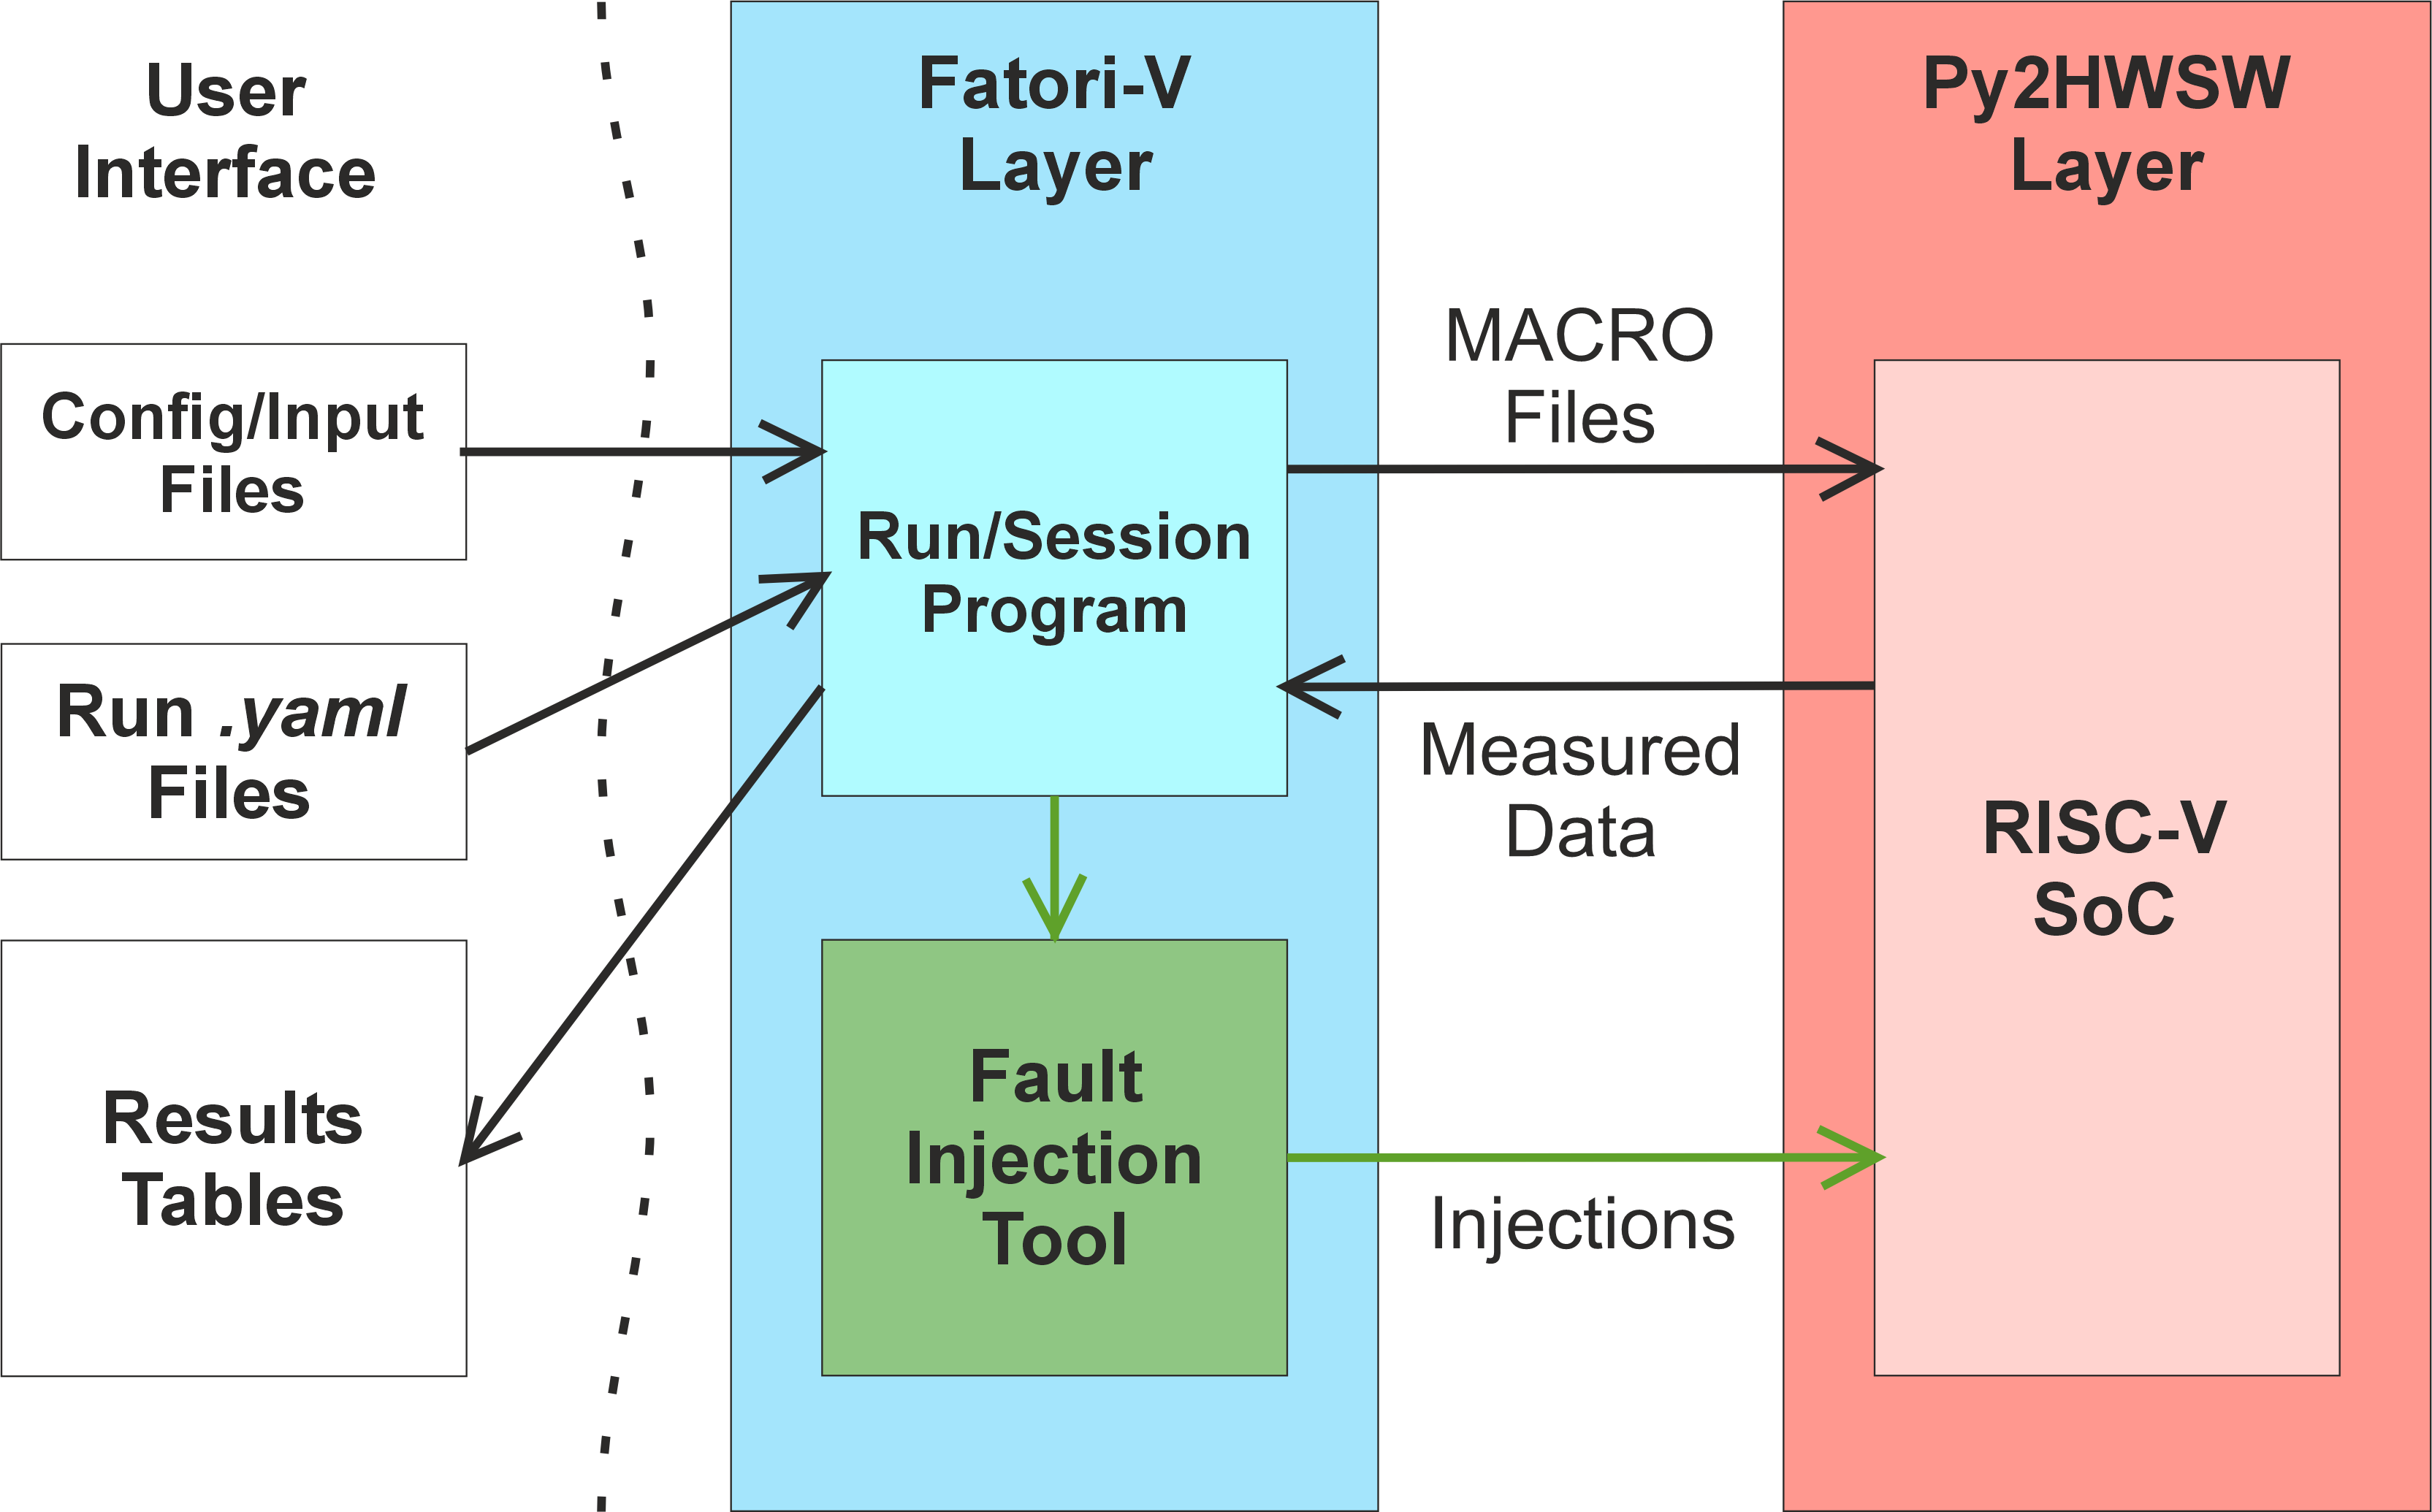
\includegraphics[width=0.7\textwidth]{Images/chap3_layers_simple.png}
    \caption{Fatori-V Overview}
    \label{fig:fatori_simple_overview}
\end{figure}


\ac{Fatori-V} is an open-source Python platform designed to support the implementation and evaluation of \acp{FTM}. It allows users to run experiments on a \ac{RISC-V} \ac{SoC} by providing a simple, compact, human-readable \ac{UI} and automating the remaining steps. \Cref{fig:fatori_simple_overview} displays its two-layer system and the main components involved.

The user sets up the platform using input and configuration files. For each
experiment, a \texttt{.yaml} file is needed. \ac{Fatori-V} generates macro
files, which are header files for SystemVerilog, firmware, benchmark
configuration, and auxiliary scripts such as Vivado TCL hooks.

The Py2HWSW layer compiles the design, produces the bitstream, and programs
the \ac{FPGA}. The platform executes benchmark sessions on the board and, when
enabled, synchronizes them with an \ac{FI} campaign, collecting logs and
creating results tables. One run represents one architecture configuration,
which contains one session for each benchmark software executing in that
architecture. Some other features of \ac{Fatori-V} are described below.
Fatori-V is an open-source Python platform engineered to facilitate the
implementation and evaluation of Fault Tolerance Mechanisms (FTMs) within RISC-V
System-on-Chip (SoC) architectures. By providing a compact, human-readable
interface that automates complex workflows, the platform streamlines the
execution of experiments on FPGA hardware. As illustrated in Figure 3.1, the
system architecture operates across two primary layers, managing the transition
from user-defined configurations to automated hardware deployment and data
collection.

The operational workflow begins with the user providing input and configuration
files, specifically through .yaml files. Fatori-V interprets these files to
generate the necessary macro headers for SystemVerilog, firmware, benchmark
configurations, and auxiliary Vivado TCL scripts. Subsequently, the Py2HWSW
layer automates the compilation, bitstream generation, and FPGA programming
processes. During execution, the platform orchestrates benchmark sessions and
integrates optional Fault Injection (FI) campaigns, capturing logs and
synthesizing results into structured tables. Within this framework, a single
"run" represents a specific architecture configuration, encompassing multiple
benchmark sessions to ensure comprehensive testing.

The platform offers extensive configurability across four primary
domains. First, Architectural Configuration allows users to define performance
features such as Instruction Cache settings and RISC-V ISA
extensions. Additionally, it provides control over monitor depth and enables
dynamic sizing of PBlocks for native Ibex modules, allowing for precise control
over logic utilization.

Second, the Fault Tolerance and Injection capabilities support the selection and
parameterization of both native Ibex and platform-specific FTMs, including
M-of-N redundancy schemes. Complementing this, the Fault Injection module allows
for temporal and spatial distribution of errors—ranging from uniform to burst
distributions across various hardware targets—enabling unified injection into
both configuration memory and registers.

Third, the Batch Execution and Automation features maximize efficiency and
reproducibility. The platform supports sequential batch processing of
experiments and multiple benchmark sessions per run. Features such as fixed-seed
trees, input auto-fixes, and "dry mode" debugging ensure that experiments remain
reliable and traceable. Users can also incorporate standard benchmarks, such as
CoreMark and Embench-IoT, or provide file overrides to bypass specific build
steps.

Finally, the Data Logging and Reporting functionality automates the storage of per-run and per-session logs, governed by configurable verbosity levels and centralized message control. It facilitates performance analysis by exporting results to .csv and .xlsx formats, mirroring build artifacts for future inspection, and calculating derived metrics through centralized configuration files.

% -------------------------------------------------------------
\section{Implementation Layers and Platform Structure}
\label{chap3:hwvssw}

\ac{Fatori-V} is built around two distinct implementation layers, as illustrated in \cref{fig:fatori_simple_overview}. The \ac{Fatori-V} Layer is the software component: it reads the user's run file, generates the interface files that configure the hardware, drives the build toolchain, orchestrates benchmark execution, and organises the resulting metrics into result tables. The Py2HWSW Layer is the \ac{RTL} component: it contains the complete hardware source tree and accepts its configuration exclusively through those generated interface files — 6~\texttt{.svh} headers, 5~\texttt{.h} headers, and 8~\texttt{.tcl} scripts, totalling 19 files.

The two layers communicate through macro files, which are generated header files that translate user-level settings into build-time constants. The most representative of these is \texttt{fatori\_features.svh}, which acts as the primary contract between the layers: every architectural choice expressed in the run file is encoded as a macro definition that the SystemVerilog source tree evaluates at compile time. By centralising all feature toggles in a single generated header, the platform ensures the hardware is always synthesised to match the exact requested configuration, without requiring any manual edits to the \ac{RTL} sources.

\begin{lstlisting}[language=matlabfloz,caption={Example of build-time feature macros generated by the software layer.},label=lst:fatori_features]
`__FATORI_MACRO_DEF(FATORI_ICACHE, 1)
`__FATORI_MACRO_DEF(FATORI_BRANCH_PRED, 1)
`__FATORI_MACRO_DEF(FATORI_RV32M, ibex_pkg::RV32MSingleCycle)
`__FATORI_MACRO_DEF(FATORI_REGFILE, ibex_pkg::RegFileFPGA)
\end{lstlisting}

Each line in \cref{lst:fatori_features} invokes \texttt{\_\_FATORI\_MACRO\_DEF}, which expands to a conditional \texttt{\`define} or parameter assignment evaluated by the \ac{RTL} at compile time. The first two entries, \texttt{FATORI\_ICACHE} and \texttt{FATORI\_BRANCH\_PRED}, are Boolean flags set to \texttt{1}, indicating that both the instruction cache and the branch predictor are to be included in the synthesised design. \texttt{FATORI\_RV32M} is assigned the enumerated value \texttt{ibex\_pkg::RV32MSingleCycle}, selecting the single-cycle multiplier implementation of the \ac{RISC-V} M~extension. Finally, \texttt{FATORI\_REGFILE} is set to \texttt{ibex\_pkg::RegFileFPGA}, directing the processor to use the \ac{FPGA}-optimised register file backed by flip-flops rather than a generic \ac{SRAM} model. Together, these four entries encode the complete set of microarchitectural features for one experiment run.

The repository is organised into several top-level directories, as shown in \cref{fig:fatori_repo_tree}.

\begin{figure}[h]
\centering
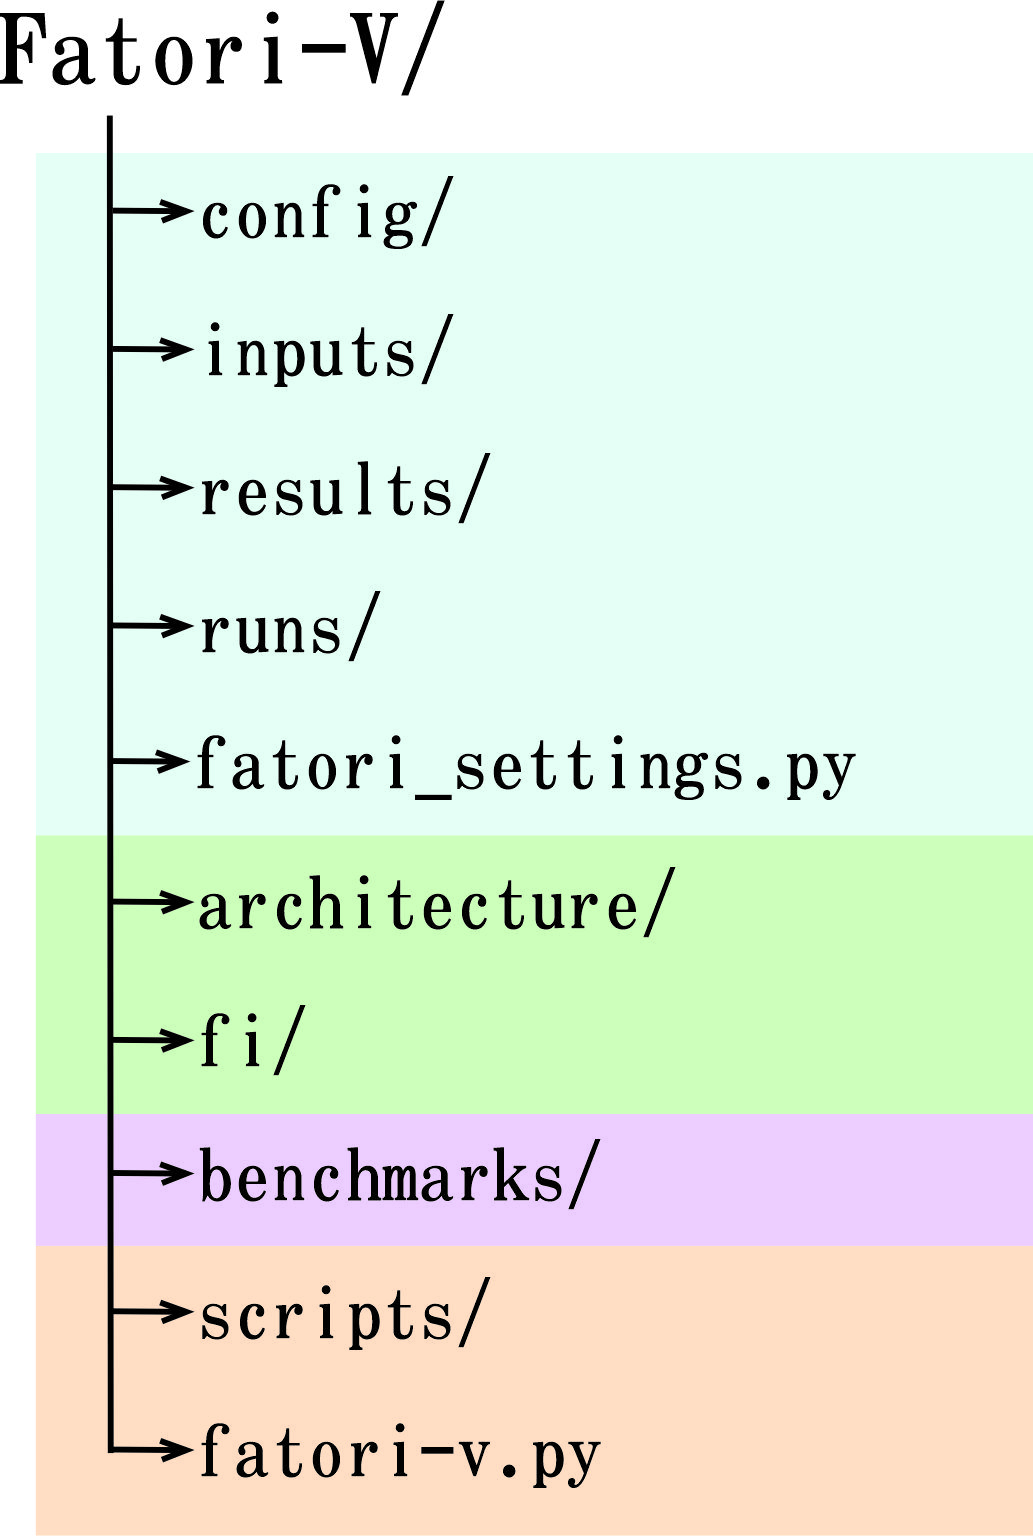
\includegraphics[width=0.27\textwidth]{Images/folder_hierarchy.jpg}
\caption{Fatori-V repository hierarchy.}
\label{fig:fatori_repo_tree}
\end{figure}

The \texttt{architecture/} directory contains the Py2HWSW layer, i.e., the complete hardware source tree. The \texttt{fi/} directory contains the \ac{FI} tool; although tightly integrated into the platform, it is implemented as a self-contained component and can also be used independently. The \texttt{benchmarks/} directory wraps the supported benchmark suites: it holds clones of the upstream repositories, Makefiles that extract and build their sources, and port files that adapt each suite to the platform. The main entry point of the platform is \texttt{fatori-v.py}, which implements the run and session control loop. The \texttt{scripts/} directory contains the supporting Python modules, organised into subdirectories by area: \texttt{cli/}, \texttt{logging/}, \texttt{reports/}, and \texttt{pblocks/}.

The user-facing directories are \texttt{runs/}, \texttt{inputs/}, \texttt{config/}, and \texttt{results/}. The \texttt{runs/} directory stores one \texttt{.yaml} experiment file per run; for each such file the platform creates a dedicated output directory under \texttt{results/}. The \texttt{inputs/} and \texttt{config/} directories, together with \texttt{fatori\_settings.py}, define the global configuration of the platform. These directories are described in detail in \cref{chap3:UI}.




% #############################################################################
\section{User Interface and Generated Outputs}
\label{chap3:UI}

\ac{Fatori-V} is controlled through a file-based \ac{UI}. Each experiment is described by a single \texttt{.yaml} run file placed under \texttt{runs/}, which selects the target board, architectural features, \acp{FTM}, benchmark sessions, optional \ac{FI} campaign, and reported metrics. A complete example is provided in \cref{app_a:yaml}. This approach keeps experiment set up at the configuration level, so the user can define and vary experiments without touching the hardware or software implementation directly. A run file is organised into three top-level blocks: \texttt{run}, which defines identification and execution context; \texttt{general}, which defines high-level switches covering hardware features, benchmarks, \ac{FI}, and metric level; and \texttt{specifics}, which defines detailed parameters for the features enabled in \texttt{general}. \Cref{tab:yaml_run_fields,tab:yaml_general_fields,tab:yaml_specifics_fields} summarise the most relevant fields.


\begin{table}[h]
\centering
\small
\setlength{\tabcolsep}{3.2pt}
\renewcommand{\arraystretch}{1.25}
\begin{tabularx}{\textwidth}{|l|X|}
\hline
Field path &
Purpose \\
\hline
\hline
\texttt{run.identification.name} &
Human-readable run name, used in output naming. \\
\hline
\texttt{run.identification.seed} &
Default seed for reproducibility. \\
\hline
\texttt{run.identification.run} &
Selects \ac{FPGA} execution or simulation mode. \\
\hline
\end{tabularx}
\caption{\texttt{run} block, identification and execution context.}
\label{tab:yaml_run_fields}
\end{table}

\begin{table}[h]
\centering
\small
\setlength{\tabcolsep}{3.2pt}
\renewcommand{\arraystretch}{1.25}
\begin{tabularx}{\textwidth}{|>{\raggedright\arraybackslash}p{0.47\textwidth}|X|}
\hline
Field path &
Purpose \\
\hline
\hline
\texttt{general.features.fault\_manager} &
Enables the Fault Manager, recommended for \ac{FI}. \\
\hline
\texttt{general.features.performance\_mechanisms.*} &
Performance feature toggles, such as \texttt{icache}, \texttt{branch\_pred}, \texttt{branch\_target\_alu}, \texttt{wstage}. \\
\hline
\texttt{general.features.isa\_extensions.*} &
\ac{ISA} toggles, such as \texttt{RV32E}, \texttt{RV32M}, \texttt{RV32B}, \texttt{RV32C}. \\
\hline
\texttt{general.features.fault\_tolerance\_mechanisms.*} &
High-level \ac{FTM} toggles, such as \texttt{dummy\_instr}, \texttt{lockstep}, \texttt{register\_m\_of\_n}, \texttt{logic\_m\_of\_n}, \texttt{self\_testing}. \\
\hline
\texttt{general.benchmarks.<bench>.enable} &
Enables a benchmark session, disabled ones are skipped. \\
\hline
\texttt{general.benchmarks.<bench>.config.*} &
Benchmark-specific parameters, when applicable. \\
\hline
\texttt{general.fault\_injection.enable} &
Enables fault injection for enabled benchmarks. \\
\hline
\texttt{general.fault\_injection.area\_profile} &
Selects the spacial injection policy (device, modules, target list, or input). \\
\hline
\texttt{general.fault\_injection.time\_profile} &
Selects the temporal injection distribution (uniform, ramp, Poisson, MMPP2, microburst, trace, or input). \\
\hline
\texttt{general.metrics\_level} &
Selects the amount of metric hardware counters included. \\
\hline
\end{tabularx}
\caption{\texttt{general} block, high-level switches and choices.}
\label{tab:yaml_general_fields}
\end{table}

\begin{table}[h]
\centering
\small
\setlength{\tabcolsep}{3.2pt}
\renewcommand{\arraystretch}{1.25}
\begin{tabularx}{\textwidth}{|>{\raggedright\arraybackslash}p{0.5\textwidth}|X|}
\hline
Field path &
Purpose \\
\hline
\hline
\texttt{specifics.ibex.*} &
Native Ibex parameter choices, such as register file and multiplier implementations. \\
\hline
\texttt{specifics.fault\_tolerance.reg\_m\_of\_n.*} &
Per-register M-of-N parameters, including N and M, correction, and targeting rules. \\
\hline
\texttt{specifics.fault\_tolerance.logic\_m\_of\_n.*} &
Logic-block M-of-N parameters, including N and M, hold, recursion control, and target selection. \\
\hline
\texttt{specifics.fault\_tolerance.self\_testing.*} &
Self-test policy, spacing, targets, and failure handling. \\
\hline
\texttt{specifics.fault\_tolerance.fault\_injection.time.*} &
Time profile parameters, such as rate, duration, and profile-specific arguments. \\
\hline
\texttt{specifics.fault\_tolerance.fault\_injection.area.*} &
Area profile parameters, such as target pool sizing, ratio rules, and target selection. \\
\hline
\end{tabularx}
\caption{\texttt{specifics} block, detailed parameters for enabled features.}
\label{tab:yaml_specifics_fields}
\end{table}


Global files, illustrated in \cref{fig:ui_inputs_config}, are configured once and reused across all experiments. The \texttt{inputs/} directory holds static hardware, firmware, and \ac{TCL} files that are copied verbatim into the build tree, with their destinations declared in \texttt{locations.yaml}; it also contains \texttt{fatori\_registers.yaml}, which assigns stable identifiers to wrapped registers, and \texttt{system\_hierarchy.yaml}, which defines parent-child relations between hardware modules for mechanisms that require hierarchical targeting. The \texttt{config/} directory governs platform behaviour: it defines the run-file validation rules, the set of measured and computed metrics together with their formulas, the event-based logging system, and global defaults such as board selection, clock frequency, and baud rate. Most defaults can be overridden through the \ac{CLI}.


\begin{figure}[h]
\centering
\begin{minipage}[t]{0.45\textwidth}
\centering
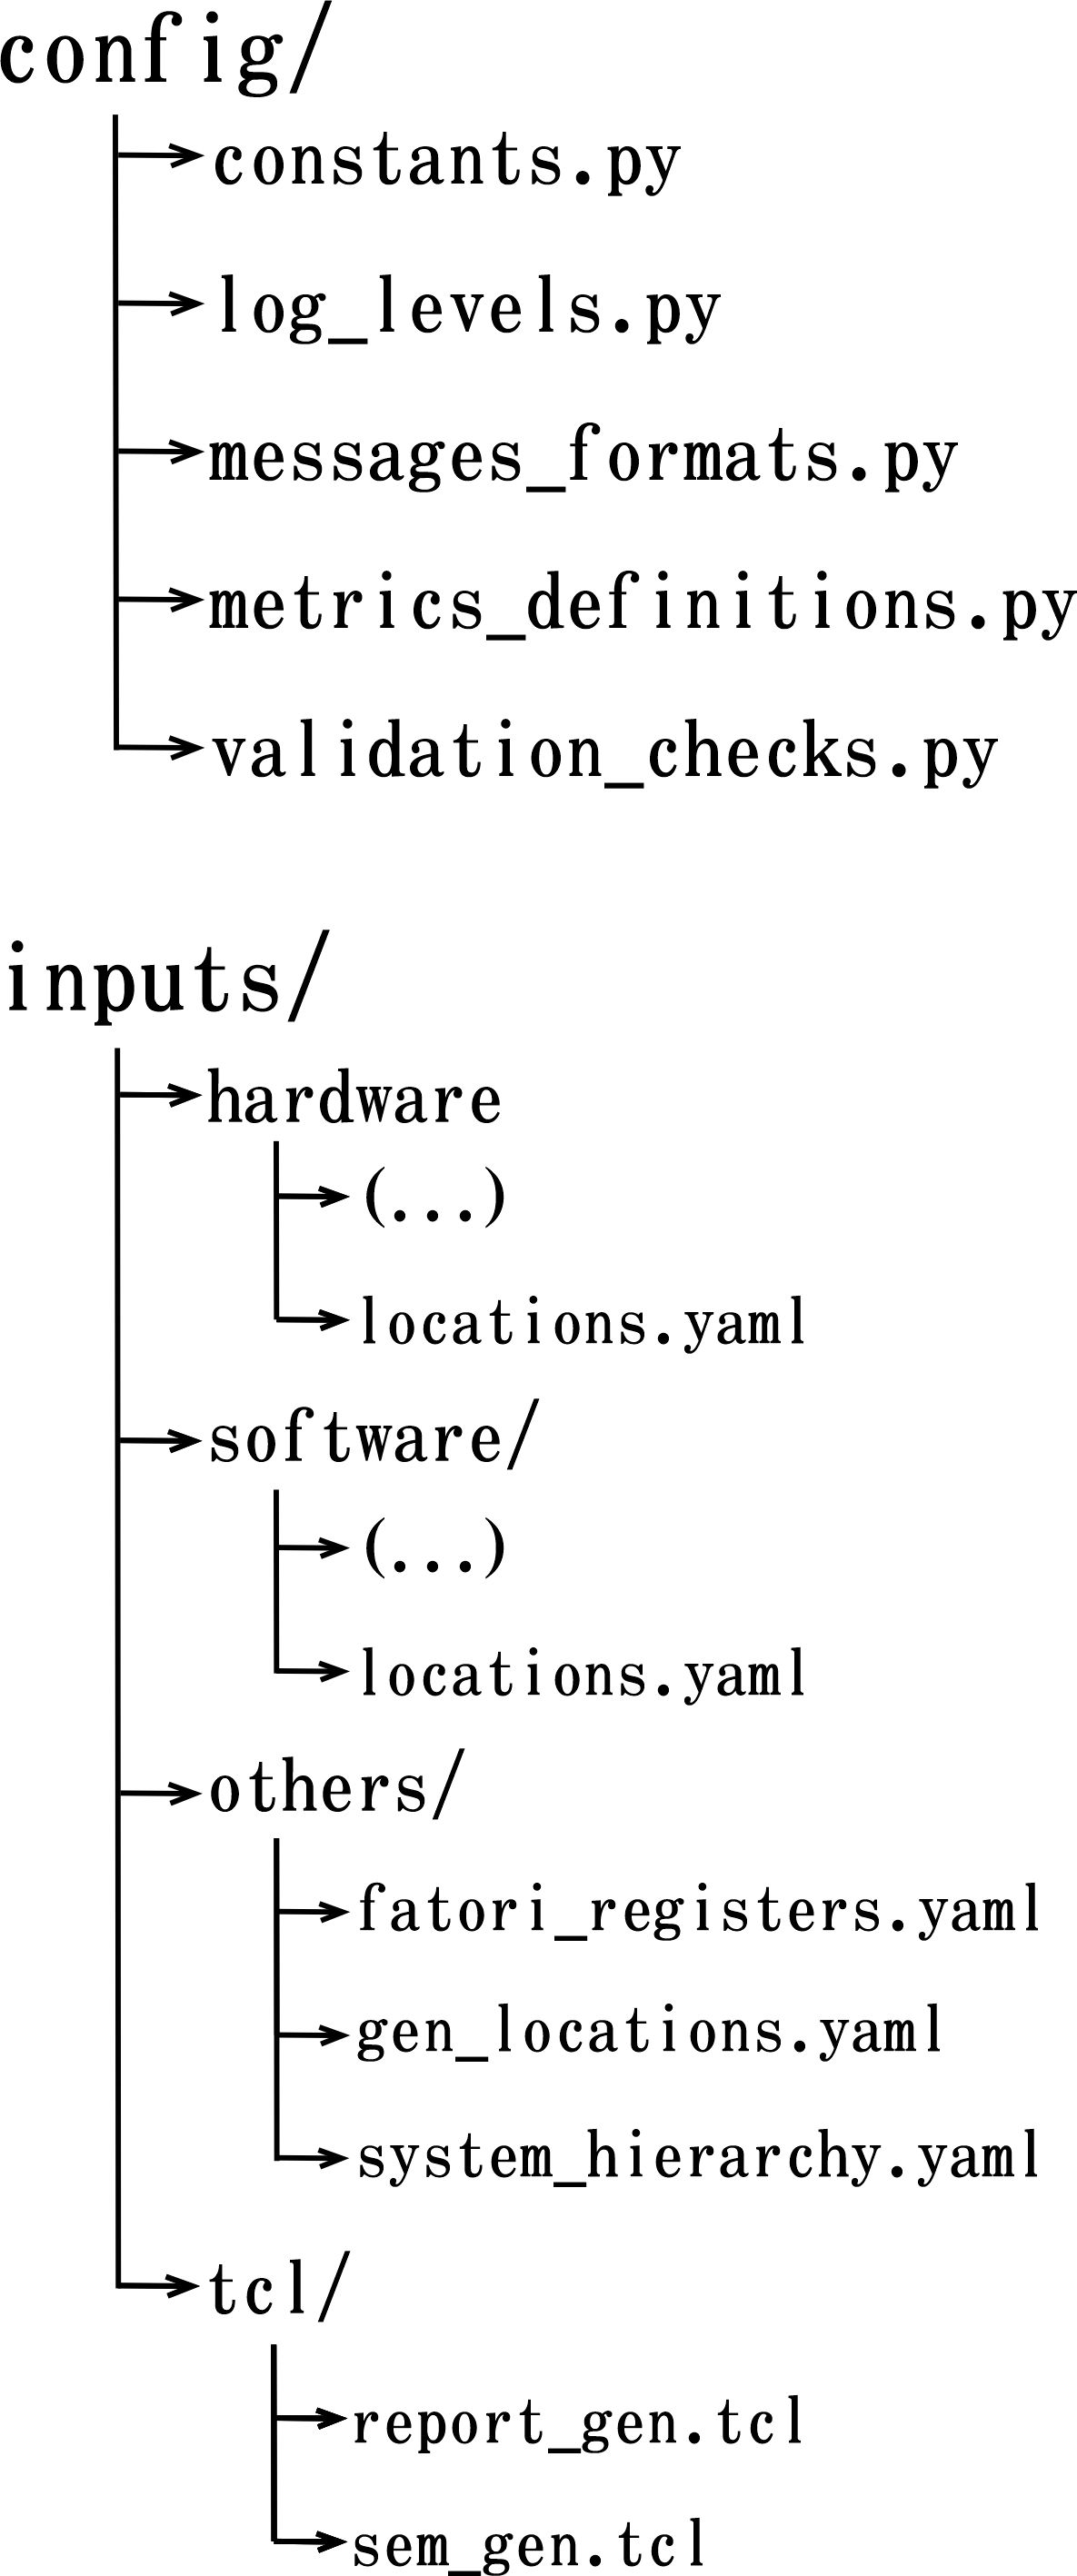
\includegraphics[width=0.5\linewidth]{Images/input_config.jpg}
\caption{Input and config entry points.}
\label{fig:ui_inputs_config}
\end{minipage}\hfill
\begin{minipage}[t]{0.5\textwidth}
\centering
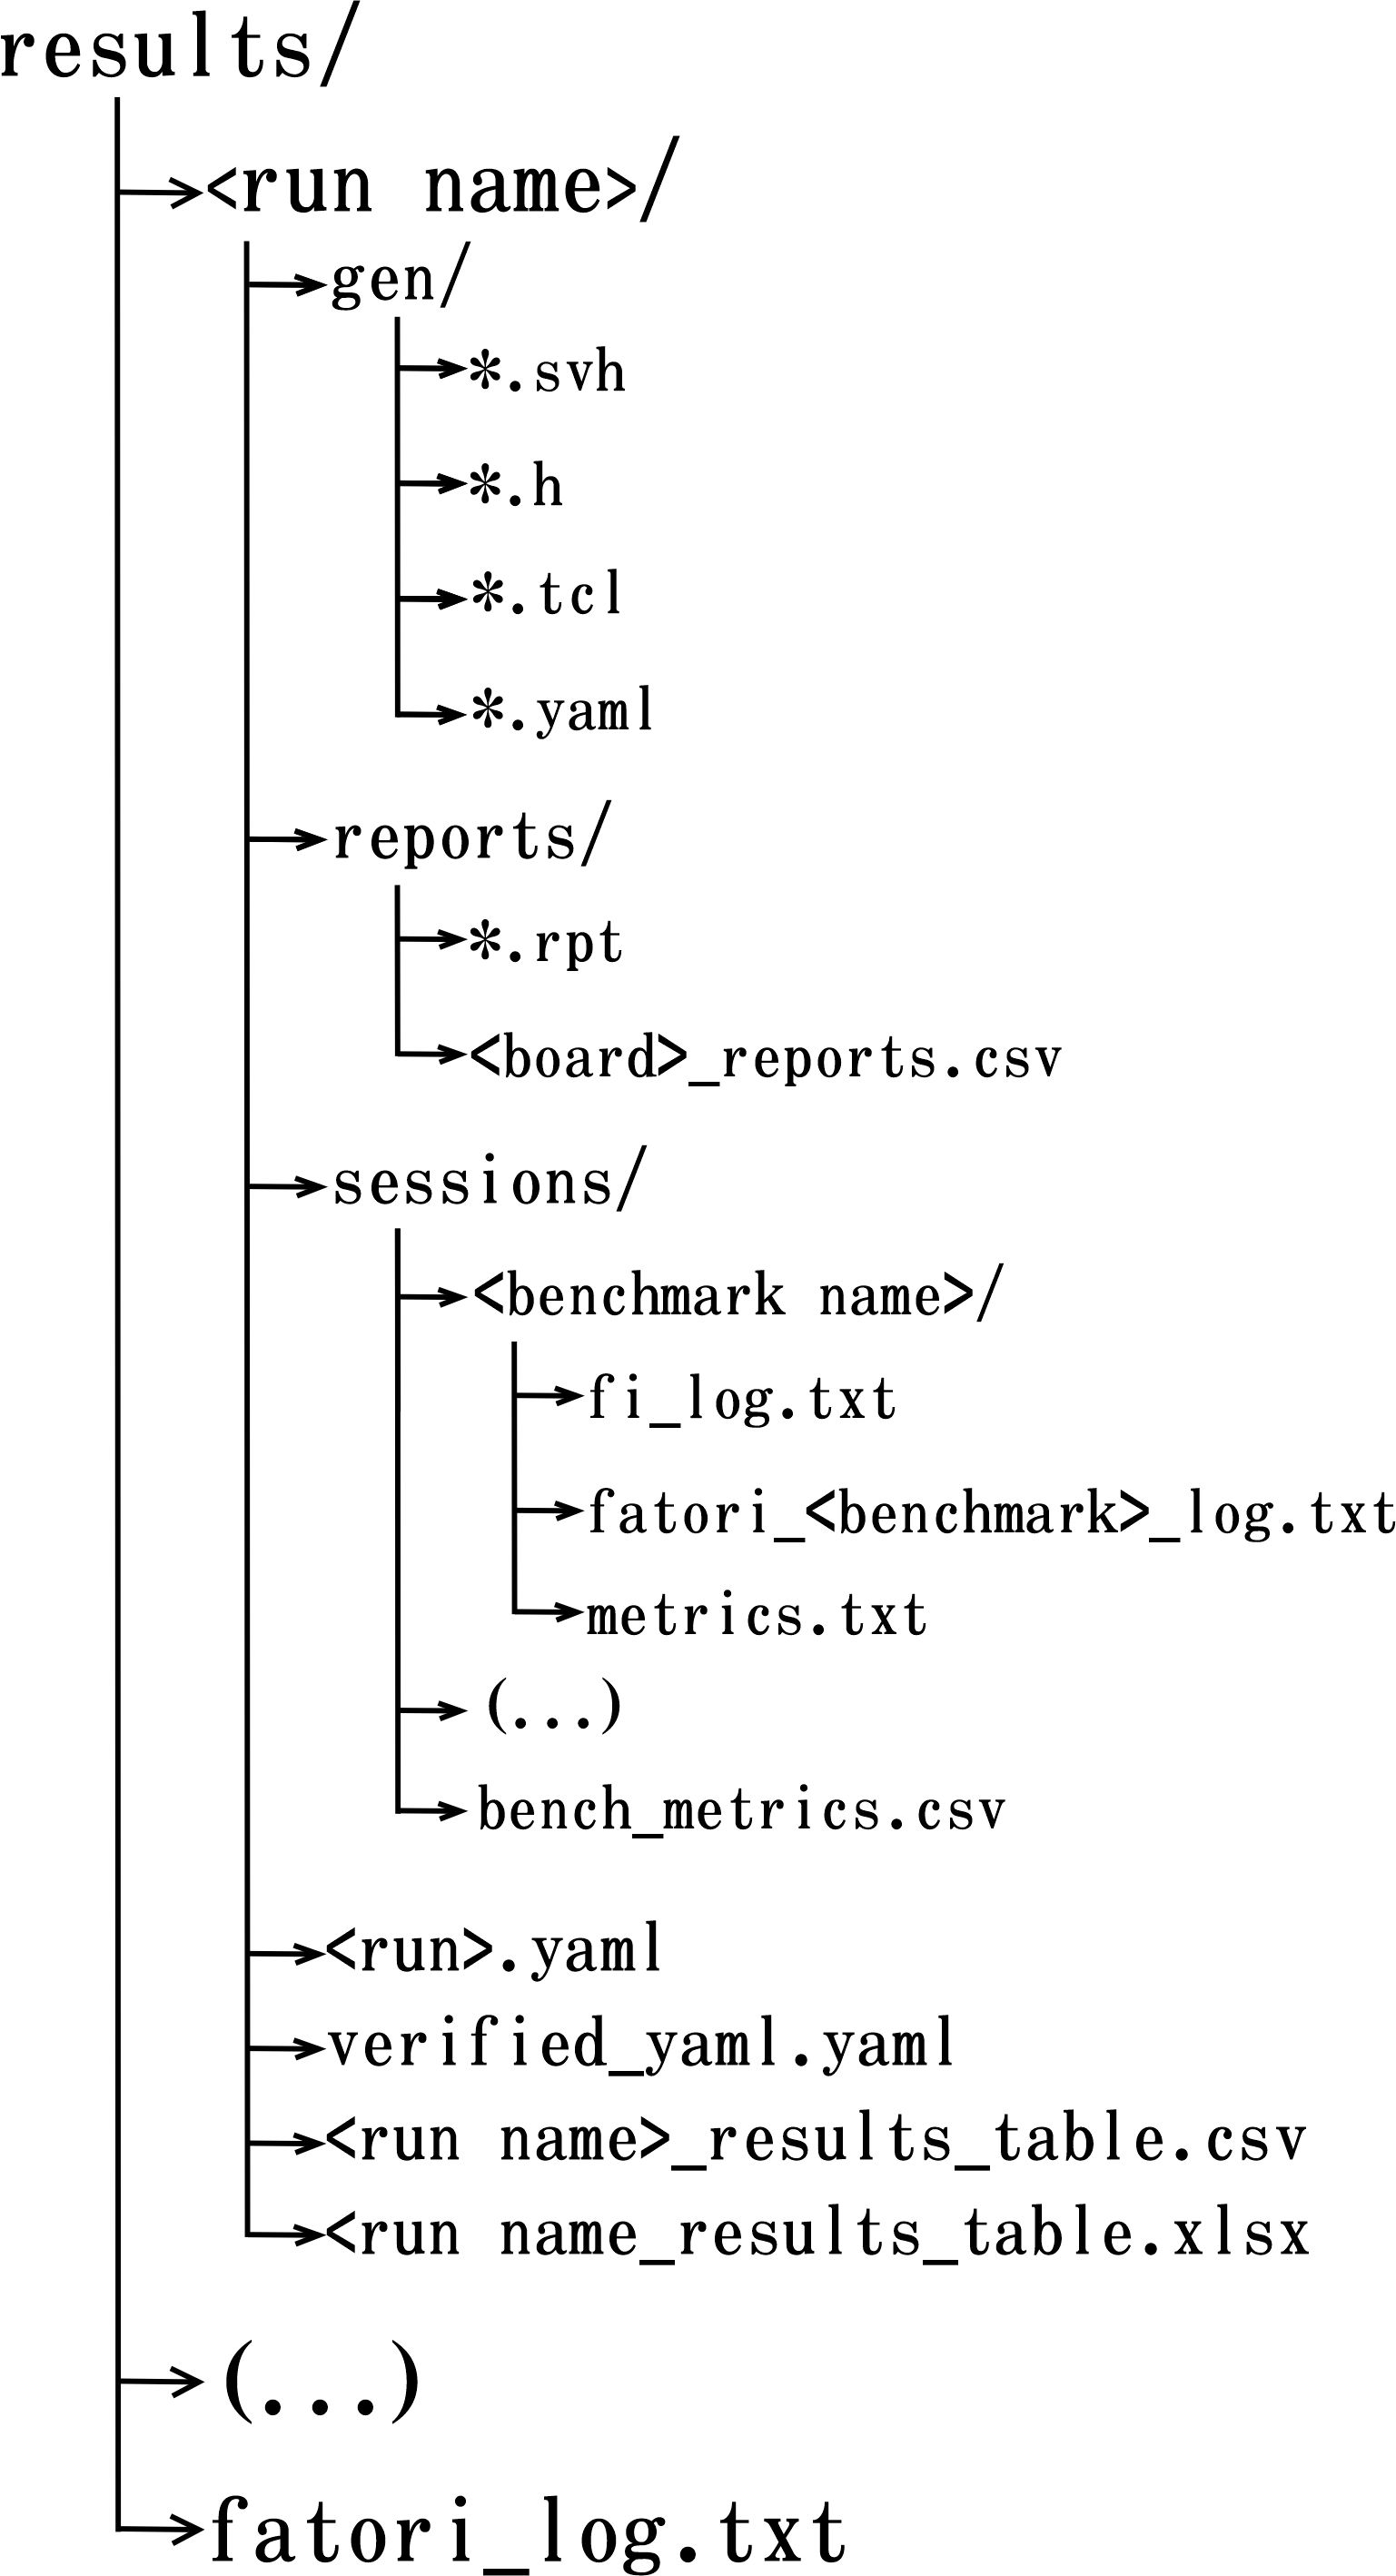
\includegraphics[width=0.6\linewidth]{Images/results.jpg}
\caption{Per-run results directory layout.}
\label{fig:ui_results_layout}
\end{minipage}
\end{figure}


Each run creates one output directory under \texttt{results/\textless run name\textgreater/}, whose structure is shown in \cref{fig:ui_results_layout}. The top level stores the original run file, the validated run file produced by the validation stage, and the consolidated \texttt{CSV} and \texttt{XLSX} result tables. The \texttt{gen/} subdirectory mirrors all files generated for that run (\texttt{.svh}, \texttt{.h}, \texttt{.tcl}, and pblock files). The \texttt{reports/} subdirectory stores Vivado build reports and the implementation metrics parsed from them. The \texttt{sessions/} subdirectory contains one directory per benchmark session, holding benchmark logs, extracted performance metrics, and \ac{FI} logs when injection is enabled.

The final output of a run is a pair of consolidated tables — a \texttt{CSV} and an \texttt{XLSX} — that merge per-session benchmark metrics with \ac{FPGA} implementation metrics parsed from Vivado reports. \Cref{tab:results_table_benchmark_excerpt,tab:results_table_fpga_excerpt} show a heavily reduced excerpt of each sheet. In Sheet~1, the primary columns of interest are the per-benchmark \ac{IPC} values and the hardware performance counters (\texttt{mcycle}, \texttt{minstret}, \texttt{hpm\_*}), which together characterise the execution behaviour of each architecture configuration. In Sheet~2, \ac{LUT} utilisation and \ac{WNS} are the key indicators of area cost and timing closure respectively.


\begin{table}[h]
\centering
\scriptsize
\setlength{\tabcolsep}{3.2pt}
\renewcommand{\arraystretch}{1.25}
\begin{tabularx}{\textwidth}{|X|X|X|X|X|}
\hline
System Features &
FI Parameters &
coremark &
embench-iot &
fatori stress \\
\hline
\hline
&
&
FI Status: on &
FI Status: off &
FI Status: off \\
\hline
Run Name: example &
FI Corrector: N/A &
instructions\_per\_cycle: 0.273 &
instructions\_per\_cycle: 0.302 &
instructions\_per\_cycle: 0.184 \\
\hline
Global Seed: 5432 &
Time Profile: uniform &
detected\_injections: 542 &
detected\_injections: 0 &
detected\_injections: 0 \\
\hline
Run Mode: fpga &
Time Seed: uses global &
mcycle: 707200229 &
mcycle: 4837000757 &
mcycle: 11558370 \\
\hline
Metrics Level: 5 &
Uniform: Rate Hz: 5.0 &
minstret: 193058420 &
minstret: 1463227089 &
minstret: 2124519 \\
\hline
Fault Manager: on &
Uniform: Period s: None &
hpm\_lsu\_busy: 95738778 &
hpm\_lsu\_busy: 490864005 &
hpm\_lsu\_busy: 2423267 \\
\hline
Dummy Instructions: off &
Area: Repeat Targets: off &
hpm\_loads: 32646654 &
hpm\_loads: 173880082 &
hpm\_loads: 689186 \\
\hline
Logic M-of-N: on &
Area: Seed: uses global &
hpm\_br\_taken: 23406924 &
hpm\_br\_taken: 85672174 &
hpm\_br\_taken: 343518 \\
\hline
\end{tabularx}
\caption{Example and heavily reduced portion of the results table (Sheet 1: Benchmark Metrics).}
\label{tab:results_table_benchmark_excerpt}
\end{table}

\begin{table}[h]
\centering
\scriptsize
\setlength{\tabcolsep}{3.2pt}
\renewcommand{\arraystretch}{1.25}
\begin{tabularx}{\textwidth}{|X|X|X|X|X|X|}
\hline
Common Info &
Utilization &
Timing &
Power &
Methodology &
DRC \\
\hline
\hline
Vivado: v.2020.2 &
Used LUTs: 4678 &
WNS: 2.571 &
OnChip Pw (W): 0.589 &
Metho Violat: 64 &
Violations: 13 \\
\hline
Date: Feb 1 2026 &
Total LUTs: 242400 &
TNS: 0.000 &
DPower (W): 0.108 &
SYNTH-15: Warning &
AVAL-318: Warning \\
\hline
Design: iob\_aes\_ku040 &
LUTs Util \%: 1.93 &
TNS Fail Endpoints: 0 &
Static Power (W): 0.481 &
SYNTH-15 Desc: ... &
AVAL-318 Desc: ... \\
\hline
Dvc: xcku040-fbva676 &
FF Total Used: 2656 &
Total Endpoints: 9849 &
DPower \%: 18.3 &
SYNTH-15 Count: 64 &
AVAL-318 Count: 1 \\
\hline
D State: Fully Routed &
Avail FF: 484800 &
WHS: 0.011 &
Static Power \%: 81.7 &
T Warn Violat: 64 &
DPIP-2: Warning \\
\hline
&
DDs Utilization \%: 0.55 &
THS: 0.000 &
&
&
DPIP-2 Desc: ... \\
\hline
\end{tabularx}
\caption{Example and heavily reduced portion of the results table (Sheet 2: FPGA Reports).}
\label{tab:results_table_fpga_excerpt}
\end{table}
